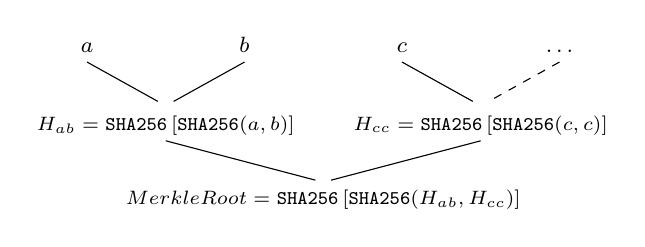
\begin{tikzpicture}[domain=-6:6,scale=1, every node/.style={scale=1}]

% 1st level
\draw[color=black, -] (-5,5) -- (-4.1,4.5); 
\draw (-5,5)node[above]{\footnotesize{$a$}};
\draw[color=black, -] (-3,5) -- (-3.9,4.5);
\draw (-3,5)node[above]{\footnotesize{$b$}};

\draw[color=black, -] (-1,5) -- (-0.1,4.5);
\draw (-1,5)node[above]{\footnotesize{$c$}};
\draw[color=black, -, dashed] (1,5) -- (0.1,4.5);
\draw (1,5)node[above]{\footnotesize{$\dots$}};

% 2nd level
\draw[color=black, -] (-4,4) -- (-2.1,3.5);
\draw (-4,3.95)node[above]{\scriptsize{$H_{ab}=\texttt{SHA256}\left[\texttt{SHA256}(a,b)\right]$}};
\draw[color=black, -] (0,4) -- (-1.9,3.5);
\draw (0,3.95)node[above]{\scriptsize{$H_{cc}=\texttt{SHA256}\left[\texttt{SHA256}(c,c)\right]$}};

\draw (-2,3.5)node[below]{\scriptsize{$\text{Merkle Root}={}\texttt{SHA256}\left[\texttt{SHA256}(H_{ab},H_{cc})\right]$}};
\end{tikzpicture}